\section{Data Simulation}\label{sec:dataset}
To test the performance of the algorithms simulated data, corresponding to the model $\textbf{Y}=\textbf{A}\textbf{X}$, is needed. All data sets are simulated based on the following approach, satisfying the sufficient conditions for recovery, displayed in theorem \ref{th:conditions}.
 
A source matrix $\mathbf{X} \in \mathbb{R}^{N \times L}$ is constructed, such that each row makes an independent signal which varies over $L$ time samples or a zero row. As such the non-zero rows of $\mathbf{X}$ are mutually orthogonal, which fulfils the first conditions of theorem \ref{th:conditions}.   
Then a mixing matrix $\mathbf{A} \in \mathbb{R}^{M \times N}$ is constructed with equally distributed and independent entries. As such the source signals are randomly mixed and the mixing matrix fulfils the second condition of theorem \ref{th:conditions}.
With known $\mathbf{A}$ and $\mathbf{X}$ the measurement matrix $\mathbf{Y} \in \mathbb{R}^{M \times L}$ is simulated according to the model, by the matrix product $\mathbf{Y} = \mathbf{AX}$.  

Two different kinds of data sets are simulated.
One simple data set with simple and predictable source signals to ensure a solution and easy visualization.
Another data set with randomised and fluctuating source signals to resemble realistic EEG measurements.

\subsection{Simple Data Set}\label{subseg_simpledata}
Two different simple data sets are simulated, with a different number of zero rows. 
One specified by $N = 5$, $k = 4$, $M = 3$ and $L = 1000$. That is a source matrix $\mathbf{X}$ with $4$ independent signals and $1$ zero row which is mixed into a data set with $3$ measurement per sample.  
The second is specified by $N = 8$, $k = 4$, $M = 3$ and $L = 1000$. This is 3 additional zero rows.
From the specifications the first data set comply to $N \leq \frac{M(M+1)}{2}$ which imply the use of Cov-DL2.
The second data set comply to $N > \frac{M(M+1)}{2}$ and $k \leq \frac{M(M+1)}{2}$ implying the use of Cov-DL1. As such it is possible to test both branches of the Cov-DL algorithm. 
     
The 4 independent source signals of $\mathbf{X}$ are defined by 
\begin{itemize}
\item[1.] a sinus signal $\sin(2t)$
\item[2.] a sawtooth signal with period $2 \pi t$
\item[3.] a sinus signal $\sin(4t)$
\item[4.] a sign function of a sinus signal $\sin(3t)$
\end{itemize}
with $t$ being a time index defined in the interval $[0,4]$ with $L$ samples. Each of the four signals are randomly drawn and used to construct a source matrix $\mathbf{X}$ of size $k \times L$, then zero rows are inserted randomly, such that $\mathbf{X} \in \mathbb{R}^{N \times L}$. 
The mixing matrix $\mathbf{A}$ of size $M \times N$ is randomly generated from a Gaussian distribution. 
By multiplying the source matrix and the mixing matrix the measurement matrix $\mathbf{Y}$ is achieved.
The simple data set then consist of $\{ \mathbf{Y}, \mathbf{X}, \mathbf{A} \}$.
In figure \ref{fig:simple} the first simple data set is illustrated by the source signals plotted over the measurement signal $\mathbf{Y}$. This illustrates how the sources signal are transformed by the mixing matrix $\mathbf{A}$.
\begin{figure}[H]
\centering
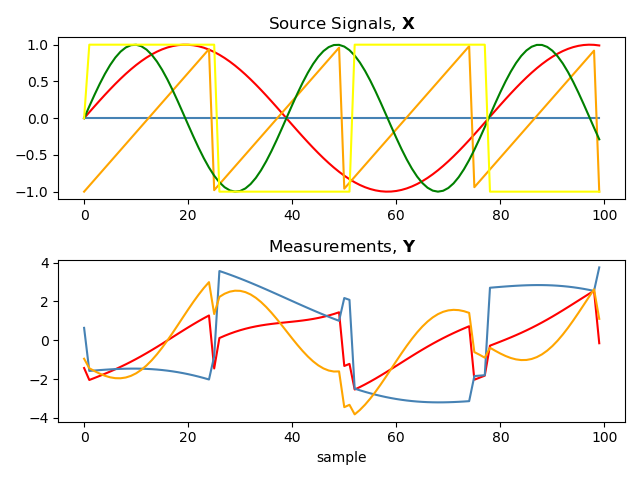
\includegraphics[scale=0.5]{figures/ch_6/simple_data.png}
\caption{Visualization of the source signals $\mathbf{X}$ in comparison to the measurements $\mathbf{Y}$ from the simple data set with $N = 5, M = 3$, $k = 4$ and $L=100$.}
\label{fig:simple}
\end{figure}
\noindent

\subsection{Autoregressive Data Set}
The purpose of this second kind of data is to resemble EEG measurements for which the model is intended. Here different data sets are simulated depending on the chosen specifications of $N$, $k$, $M$ and $L$. 
Every data set is constructed based on four different autoregressive processes each representing a source signal:
\begin{itemize}
\item[-] $x_{1}^{t} = \sum_{i=1}^{2} \phi_i x^{t-i} + w_t$
\item[-] $x_{2}^{t} = \sum_{i=1}^{2} \zeta_i x^{t-i} + w_t$
\item[-] $x_{3}^{t} = \sum_{i=1}^{3} \eta_i x^{t-i} + w_t$
\item[-] $x_{4}^{t} = \sum_{i=1}^{4} \xi_i x^{t-i} + w_t$
\end{itemize}
where $\boldsymbol{\phi}, \boldsymbol{\zeta}, \boldsymbol{\eta}$ and $\boldsymbol{\xi}$ are different model parameters and $w_t$ is white noise.
$\mathbf{X}$ is constructed by drawing $k$ autoregressive processes randomly among the four, if $k < N$ zero rows are inserted randomly such that $\mathbf{X} \in \mathbb{R}^{N \times L}$  
The mixing matrix $\mathbf{A}$ of size $M \times N$ is, like the previously, generated randomly from a Gaussian distribution.
By multiplying the source matrix and the mixing matrix the measurement matrix $\mathbf{Y}$ is achieved.
The autoregressive data set then consist of $\{ \mathbf{Y}, \mathbf{X}, \mathbf{A} \}$. 

One simulation of the autoregressive data set is illustrated in figure \ref{fig:AR}. The data set specified by $N = 5$, $M = 3$, $k = 4$ and $L = 1000$.
\begin{figure}[H]
\centering
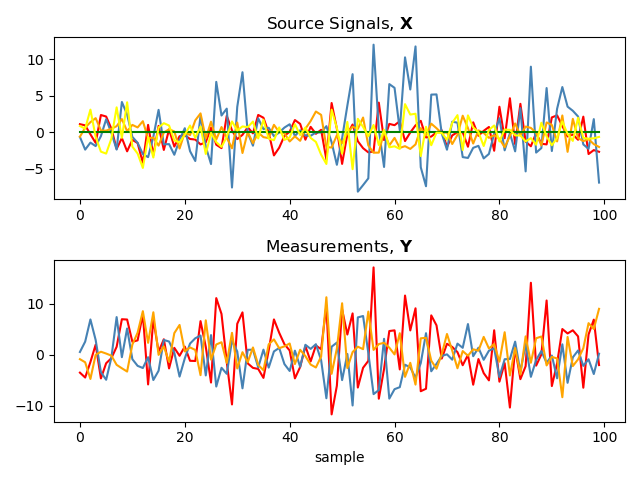
\includegraphics[scale=0.5]{figures/ch_6/AR_data.png}
\caption{Visualization of the source signals $\mathbf{X}$ in comparison to the measurements $\mathbf{Y}$ from an autoregressive data set specified by $N = 5$, $M = 3$, $k = 4$ and $L=1000$. For simplicity only samples [0:100] are plotted.}
\label{fig:AR}
\end{figure}
\noindent

